%% LaTeX2e class for student theses
%% sections/content.tex
%% 
%% Karlsruhe Institute of Technology
%% Institute for Program Structures and Data Organization
%% Chair for Software Design and Quality (SDQ)
%%
%% Dr.-Ing. Erik Burger
%% burger@kit.edu
%%
%% Version 1.3.6, 2022-09-28

\chapter{Background}
\label{ch:Background}

We provide an overview of the background knowledge necessary to understand the following chapters in this chapter. We start with
active learning, describing common active learning settings. Next, we cover continual learning, including conventional continual learning
scenarios and a taxonomy of continual learning methods. Finally, we describe model stealing attacks, introduce the most relevant terminology,
and outline model stealing defenses.


\section{Active Learning}
\label{sec:ActiveLearning}

\gls{al} is a subfield of machine learning that focuses on the problem of how to select the most informative data points to label.
Research in \gls{al} is motivated by the contrast between low-effort data acquisition and resource-intensive labeling.
Therefore, the objective of active learning research is to create techniques that optimize model performance while minimizing the amount of
labeled data required. A typical \gls{al} scenario comprises a learner, an oracle, unlabeled samples, and labeled data. The learner
itself is then the \gls{ml} model. Let $I$ be the instance space (i.e., the set of all possible data points), and $L$ be the label
space (i.e., the set of all possible labels). The oracle $O$ represents the function
\begin{equation}
    O: I \rightarrow L, x \mapsto y(x)
\end{equation}
where $y(x)$ is the true label of the data point $x$. In the following, we will use $y$ as a short form of $y(x)$. $U$, the set of unlabeled data,
is a subset of $I$ just as the set of labeled data $L$. In the beginning, there are no labeled data points. Often a few labeled data points
are randomly sampled from $U$ and labeled by the oracle to initialize the learning process. A detailed overview of research activities within
the active learning domain is presented by Settles \cite{settles2009active}. Note, however, that more recent works are not contained in this
literature survey because it was last updated in 2009. In general, \gls{al} methods can be divided into three categories:
\begin{itemize}
    \item \textbf{Query Synthesis Active Learning}
    \item \textbf{Pool-based Active Learning}
    \item \textbf{Stream-based Active Learning}
\end{itemize}
While researchers generally agree on this data-centric taxonomy, it is worth noting that the type of \gls{ml} model used
(e.g. (convolutional) neural networks or support vector machines) and the type of data used (such as images or text) play a decisive role in the
effectiveness of an \gls{al} strategy. An example of this is the pool-based \gls{al} strategy CoreSet \cite{sener2017active}, which
was designed to suit the requirements of \glspl{cnn}.

\subsection{Query Synthesis Active Learning}
\label{sec:QuerySynthesisActiveLearning}
Query synthesis active learning, also known as membership query synthesis active learning, was among the first \gls{al} scenarios proposed
\cite{angluin1988queries}. Query synthesis methods synthesize data points from the input space instead of sampling real data points. Modern query
synthesis methods train a generative model (e.g., a Generative Adversarial Network) \cite{zhu2017generative}
which learns the distribution of unlabeled data. However, earlier works relied on statistical models such as Gaussian mixture models 
\cite{cohn1996active}. The generated queries are then labeled by the oracle and can be used to train the machine learning Model. Note that
query synthesis is not limited to classification tasks. For example, Cohn et al. \cite{cohn1996active} proposed a method to predict the absolute coordinates
of a robot hand when given the joint angles of its mechanical arms as inputs. When the oracle is a human annotator, query synthesis active learning
researchers have encountered problems in labeling them. Human annotators struggled to assign any class to them in the survey of Baum et al. \cite{baum1992query}
because the generated queries do not show any class-discriminative features.

% TODO: Hier ein Bild wie QS Active Learning funktioniert einfügen

\subsection{Pool-based Active Learning}
\label{sec:PoolBasedActiveLearning}
Pool-based active learning is the most widely studied and used type of active learning. The idea behind pool-based active learning approaches
is to iteratively select the most informative data points from the current unlabeled pool, query the oracle for their labels and add them to the
labeled pool. Next, the \gls{ml} model is trained on the current labeled pool. This process repeats itself until the query budget is exhausted.
A more detailed explanation can be found in algorithm \ref{alg:PoolBasedActiveLearning}. More formally, the pool-based active learning problem
can be defined as:
\begin{equation}
    \min_{s^1 \subseteq U: |s^1| \leq b} E_{x,y \sim P_{(X,Y)}}[\mathcal{L}(x,y;L \cup b)],
\end{equation}
where $U$ is the unlabeled pool, $b$ is the query batch size and $L$ is the labeled pool.
In other words, a pool-based active learning algorithm aims to select the points that minimize the expected loss of the model on the labeled pool when
being added to it. As can be seen from  algorithm \ref{alg:PoolBasedActiveLearning}, the structure across pool-based active learning strategies is similar.
The main difference between these is the informative measure, i.e., the criterion with which they select the data points to label next. Within 
pool-based active learning, there are two subcategories: uncertainty-based sampling and diversity-based sampling. 
Uncertainty-based sampling strategies select the data points that the model is most uncertain about. Diversity-based sampling strategies, on the other
hand, aim to select data points that best represent the data distribution in the unlabeled pool.

\begin{algorithm}
    \caption{Pool-based Active Learning} \label{alg:PoolBasedActiveLearning}
    \begin{algorithmic}[1]
        \Require Unlabeled data $U$,Labeled data $L = \emptyset$:, Oracle $O$, Model $M$, budget $B$
        \State Select $k$ data points from $U$ at random, obtain labels by querying $O$ and set $L=\{x_1,\ldots,x_1\}$
        and $U = U \setminus \{x_1,\ldots,x_1\}$ \Comment{Initialization}
        \State Train $M$ on initial labeled set $L$
        \While{label budget $B$ not exhausted}
            \State Select $l$ data points from $U$ predicted to be the most informative by the Active Learning strategy
            \State Obtain labels by querying $O$ for $x_i,\ldots,x_l$
            \State Set $L= L \cup \{x_i,\ldots,x_l\}$ and $U = U \setminus \{x_i,\ldots,x_l\}$
            \State Train $M$ on labeled set $L$
        \EndWhile
    \end{algorithmic}
\end{algorithm}

\subsection{Stream-based Active Learning}
\label{sec:StreamBasedActiveLearning}
Stream-based active learning, introduced by Cohn et al. \cite{cohn1994improving}, is closer to pool-based active learning than query synthesis
active learning. The main difference between stream-based active learning and pool-based active learning is that data arrives sequentially
instead of having a batch of data points. In the stream-based active learning scenario, the learner draws a data point from the data source
one at a time. For each data point, the learner can then decide to query the oracle for its label or to discard it. The decision whether to label a
data point can either be made based on its informativeness \cite{dagan1995committee} or its location within the instance space \cite{cohn1994improving}.
In the latter case, the learner would label the data point if it in a region of the instance space that the learner is not confident about.

\section{Continual Learning}
\label{sec:ContinualLearning}
Continual learning is a subfield of \gls{ml} that aims to solve the problem of catastrophic forgetting. Nowadays, most \gls{ml} services are deployed
in an environment where constant changes occur. To adapt to their environment, machine learning models need to learn new tasks without forgetting the knowledge
they have acquired in the past. In contrast to human behavior, the performance of \gls{mls} models on old tasks rapidly decreases when they are trained
on new tasks. This phenomenon is known as catastrophic forgetting and was already discovered in the early days of \gls{ml} research \cite{mccloskey1989catastrophic}.
Generally speaking, research in continual learning aims not only to alleviate catastrophic forgetting but to solve the 
\enquote{stabiliy/plasticity dilemma} \cite{carpenter1988art}. The stability/plasticity dilemma refers to the fact that \gls{ml} models
should be stable enough to retain their performance on old tasks while simultaneously being plastic enough to adapt to new ones. This is a dilemma
because both properties are desirable even though they conflict with each other. In practice, \gls{ml} models tend to be more plastic than stable.
This is especially true for Deep Neural Networks, but generally for all \gls{ml} models trained by greedily updating their parameters using
gradient descent \cite{mundt2020wholistic}. \par
Continual learning is employed widely in scenarios where new tasks arrive or the data distribution changes over time. Despite being useful
in these classic scenarios, continual learning approaches can also be used in cases where storing data is impossible for legal reasons or due to memory
constraints, i.e., when batch learning is inapplicable. 


\subsection{Continual Learning Scenarios}
\label{sec:ContinualLearningScenarios}
Continual Learning is a rapidly evolving research field. Therefore, terminology as well as taxonomy are currently being established. Among the most
important factors to distinguish is how new tasks arrive. In the following, we will introduce the three typical Continual Learning Scenarios as
presented by van de Ven et al. \cite{van2022three}. These are Task-Incremental Continual Learning, Domain-Incremental Continual Learning and
Class-Incremental Continual Learning.

\subsubsection{Task-Incremental Continual Learning}
\label{sec:TaskIncrementalContinualLearning}
%TODO: 7.5. 2:13 hier weiter machen mit polishin
%TODO: Add a figure that shows the difference between the three scenarios. For Task-Incremental learning mention tuple with task id.
In the Task-Incremental setting, a model is informed about which task it will be trained on or which task the data whose label it is supposed to predict belongs to.
Task information is conveyed through an integer task identifier. Because the model does not have to infer the task it is supposed to predict
or learn, it is possible to have task-specific components in the model. For Neural Networks, this entails one output layer per task, whereby the corresponding
output layer is utilized for each task, while the remaining layers are shared among all tasks. These classifiers are known as \enquote{multi-head} classifiers
\cite{vandeven2019generative}. An example would be the following: The first task is to classify images of cats and dogs. The second task is to classify cows and sheep.
The model would have one output layer to classify cats and dogs and a second to classify cows and sheep. When training the first task, only the first output layer
is used. Upon the arrival of the second task, the model is retrained with the second output layer. The mapping learned is 
\begin{equation}
    f: X \times T \rightarrow Y
\end{equation}
Where $X = \mathbb{R}^{N x N x C}$ is the input space (i.e., all possible input images of size $N x N$ with $C$ channels), $T = \{1,2,\ldots\}$ is the task space (i.e., all possible
tasks that the model can be trained on) and $Y = \mathbb{Z}_{k}$ is the label space with $k$ being the number of possible classes.
% Figure with decision tree for the continual learning scenarios like in https://www.nature.com/articles/s42256-022-00568-3
\subsubsection{Domain-Incremental Continual Learning}
\label{sec:DomainIncrementalContinualLearning}
In the Domain-Incremental setting, task identities are not passed to the classifier during evaluation. Since the underlying task does not change, this is also not necessary.
While the structure of the task stays the same,  the distribution of the data changes. An example of Domain-Incremental Continual Learning would be the classification of digits
between 0 and 9 (such as those in the MNIST \cite{mnist_web} dataset) where the digits for one subtask are green and blue for the other. The mapping learned is 
\begin{equation}
    f: X \rightarrow Y
\end{equation}
Where $X = \mathbb{R}^{N x N x C}$ is the input space (i.e., all possible input images of size $N x N$ with $C$ channels), and $Y = \mathbb{Z}_{k}$ is the label space with $k$ being the
number of possible classes.

\subsubsection{Class-Incremental Continual Learning}
\label{sec:ClassIncrementalContinualLearning}
Class-Incremental Continual Learning is the most challenging scenario. Like in the Domain-Incremental setting, task identities are not provided at evaluation time. Instead, they need to
be inferred by the model. In this scenario, a classifier is exposed to multiple tasks containing different classes. An example would be again the classification of digits between 0 and 9.
Contrary to the previous setting, this time each task comprises a disjoint subset of digits. The classifier would be trained on the first task, containing the digits 0 and 1. The second task
would contain the digits 2 and 3, and so on. During the evaluation, the classifier would have to classify the digits correctly and infer which task they belong to simultaneously. 
The mapping learned is  
\begin{equation}
    f: X \rightarrow Y \times T
\end{equation}
Where $X = \mathbb{R}^{N x N x C}$ is the input space (i.e., all possible input images of size $N x N$ with $C$ channels), $T = \{1,2,\ldots\}$ is the task space (i.e., all possible
tasks that the model can be trained on) and $Y = \mathbb{Z}_{k}$ is the label space with $k$ being the number of possible classes.

\subsection{Continual Learning Approaches}
\label{sec:ContinualLearningApproaches}
The Continual Learning approaches proposed so far can be grouped into three categories according to \cite{parisi2019continual} \cite{mundt2020wholistic} and \cite{zenke2017continual}.
Parisi et al. \cite{parisi2019continual} propose to group Continual Learning approaches into \textbf{regularization}, \textbf{rehearsal}, and \textbf{architectural} approaches whereas Zenke et al.
\cite{zenke2017continual} group Continual Learning approaches into \textbf{architectural},\textbf{functional} and \textbf{structural} approaches. In the following, we will stick to the
categorization proposed by Parisi et al. because it is broader and fully encompasses the categorization by Zenke et al. Furthermore, Parisi et al.'s classification has been adopted by
recent continual learning reviews \cite{mundt2020wholistic}.

\subsubsection{Regularization Approaches}
\label{sec:RegularizationApproaches}
Regularization-based approaches to Continual Learning aim to prevent the forgetting of previous tasks by adding a regularization term to
the model's loss function. The regularization term is a proxy for how much model performance on previous tasks will decrease. A high
regularization term indicates that the model will perform poorly on the old tasks with the current weights. Consequently, a low regularization
term indicates that the model has not lost much knowledge of the old tasks. Regularization-based Continual Learning approaches are further
divided into two subgroups based on the method by which the regularization term is calculated. \par
There are \textbf{structural} approaches that regularize based on weight changes to the model and there are \textbf{functional}
approaches that regularize based model output. Structural approaches determine an importance weight for each
model parameter. Popular approaches either use Fisher Information \cite{kirkpatrick2017overcoming} \cite{lee2017overcoming} or
gradient information \cite{aljundi2018memory} \cite{zenke2017continual}.\par
Functional regularization approaches are inspired by knowledge distillation \cite{hinton2015distilling}. They add a distillation
loss to the objective function which is computed based on the prediction of a data sample stored for future use. These data samples
are called soft targets. Li et al. \cite{li2017learning} compute the distillation loss by using the output of the newly arrived task
given by the model trained on the old tasks. The distillation loss they introduce aims to retain the prediction of the old model on
the new task, even if the prediction itself may be inaccurate. Another approach uses autoencoder reconstructions of old tasks to
compute the distillation loss \cite{rannen2017encoder}.

\subsubsection{Rehearsal Approaches}
\label{sec:RehearsalApproaches}
Rehearsal approaches aim to prevent catastrophic forgetting by fitting a model's parameters to the distribution
of an incoming task and all previous tasks simultaneously. Within Rehearsal approaches it is important to remember the trade-off between
model performance and computational cost. In general, using more data from previous tasks to train the model will increase the accuracy. 
However, to train on more data, the data has to be stored and fed into the training process which is costly in terms of memory.
Training on more data can be done either by replaying stored data from previous tasks or by
retraining on generated data drawn from the distribution of previous tasks. Continual Learning Methods that rely on the former idea are
categorized as \textbf{exemplar rehearsal} approaches while those that rely on the latter idea are categorized as \textbf{generative replay}
approaches. \par
Exemplar Rehearsal techniques store data from previous tasks in a so-called \enquote{Replay Buffer}. When training on a new task $T_N$, samples
from the replay buffer are drawn and fed to the model while training on $T_N$. Approaches falling in this category vary in the way that the replay
buffer is constructed, and the way samples are replayed during training of a new task. \par
Generative Replay approaches use generative models to generate artificial samples from previous tasks. These samples are then replayed to
the model when training on a new task $T_N$. Compared to Exemplar Rehearsal approaches, Generative Replay approaches do not require a replay buffer.
However, the generative model itself needs to be stored. 

\subsubsection{Architectural Approaches}
\label{sec:ArchitecturalApproaches}
Architectural approaches aim to tackle Continual Learning by changing the underlying model architecture. Within this category, there are two  
subcategories. Approaches falling into the first category are called \textbf{Fixed Capacity} methods while the second category is called
\textbf{Dynamic Growth}. \par
Fixed Capacity methods do not change the number of model parameters but rather the parameters used for each task. They assume that parts of
the model architecture are redundant and therefore can be reused for different tasks. When training on a new task $T_N$, those parameters that are
important for the task (how importance is defined depends on the specific approach) are used to form a path through the model only used for
$T_N$. All other parameters are frozen, i.e., their weight and bias are set to 0. \par
Dynamic Growth approaches on the other hand allow adding new layers or single neurons to the model when training on a new task. The difference between
approaches falling into this category is their decision on when to add new layers or neurons. A popular criterion for deciding when to add new model
parameters is when the loss function plateaus \cite{ash1989dynamic}.

\section{Model Stealing}
\label{sec:ModelStealing}
With the advent of Machine Learning as a Service (\gls{mlaas}), an increasing amount of machine learning models are being exposed to the public via 
prediction \glspl{api}. The idea of these prediction APIs is that a user can request a prediction from a model by sending a request containing an unlabeled data
point to the \gls{api}. The response to the request is then the model's prediction for the data point. Prediction \glspl{api} are monetized by charging the user
on a pay-per-query principle. That means each request has a fixed price for each query which is usually subtracted from the account balance every month. 
Providing public access to a Machine Learning model is a win-win situation. The model developer is compensated for his or her efforts in gathering and labeling
appropriate training data. The developer also chooses a proper model architecture, trains the model, and fine-tunes its hyperparameters. On the other hand,
the user of the prediction \gls{api} can benefit from the model's predictions without having to train the model. \par
Since the developed model is the intellectual property of the model developer, it is important that only the model's predictions are exposed to the public and
not the model (i.e., its architecture and the model weights)itself. However, in the last years, numerous research papers have been published that demonstrate how
several features of a machine learning model can be extracted, i.e., its functionality \cite{tramer2016stealing}, its architecture \cite{oh2019towards} and its
training data \cite{shokri2017membership}. This newly created field of research is called \textbf{Model Stealing} or \textbf{Model Extraction}, and it is a subfield
of \textbf{Adversarial Machine Learning} according to Oliynyk et al. \cite{oliynyk2022know}. Because Model Extraction attacks are so effective, further research
concerning model stealing defense mechanisms has been published. In the following, we will use the taxonomy provided by Oliynyk et al. (see Figure 
\ref{fig:ModelStealing:Taxonomy}) \cite{oliynyk2022know} as a basis for our categorization of Model Stealing attacks and defenses.

\subsection{Terminology}
\label{sec:ModelStealing:Terminology}
Since Model Stealing is a fairly new field it comes with numerous terms that are not commonly used in other fields of Machine Learning and others that are used 
synonymously. To avoid confusion, we will define and explain the terms we use in this section and. \par
\textbf{Model Stealing Attack}: The process of maliciously querying a machine learning model to extract some or all of the model's features, such as its
architecture, its weights or its training data. Model Stealing Attacks are also known as Model Extraction Attacks or Model Inference Attacks among others. \par
\textbf{Target Model}: The model queried via the prediction \gls{api} and whose features the attacker aims to extract. The target model is also referred to as Oracle, Victim Model, or Secret Model. \par
\textbf{Substitute Model}: The model used by the attacker to extract the target model's features. Synonyms for Substitute Model are Adversarial Classifier,
Knockoff Model or Inferred Model. \cite{orekondy2019knockoff} have demonstrated that is favorable to choose a rather complex model architecture which is in line with 
our findings.\par
\textbf{Target Model Dataset}: The dataset that the target model has been trained on. The term Target Model Dataset has not been used in the literature before (to 
the best of our knowledge). However, we choose this term over the synonymous term Secret Dataset because we believe it is more expressive. During Model Stealing Attacks,
the attacker has no access to the target model's dataset, i.e., it is kept secret. For research purposes, however, a test set of the Target Model Dataset is
used to evaluate the performance of the Substitute Model. \par
\textbf{Thief Dataset}: The dataset used by the attacker to train the Substitute Model. The Thief Dataset is also known as Fake dataset, Attacker Set or 
Transfer Set. When constructing the Thief Dataset, the attacker can either use \textbf{Natural Non-Problem Domain} (\gls{nnpd}) or \textbf{Synthetic Non-Problem Domain} (\gls{snpd})
data. \gls{nnpd} data is data that is collected from the real world but does not (knowingly) overlap with the Target Model Dataset whereas \gls{snpd} data is artificially created,
usually by drawing from a given distribution such as a multidimensional Uniform Distribution \cite{pal2020activethief}. Empirical observations show that using \gls{nnpd} data
yields significantly better results than using \gls{snpd} data. Even when using \gls{nnpd} data, significant differences between different datasets have been observed 
\cite{pal2020activethief}. In general, it is wise to choose a dataset that is as diverse as possible. Regardless of using \gls{snpd} or \gls{nnpd} data, the adversary should keep the
dimensions of the Target Model Dataset, i.e., image size and especially the number of channels for image datasets, in mind and adapt the Thief Dataset accordingly. \par
\textbf{Agreement}: The relative agreement between the predictions of the Substitute Model and the Target Model. The agreement is computed on a test set of the Target 
Model dataset, meaning that it is not accessible by the attacker. The agreement is also known as Extraction accuracy, label prediction match, or similarity. More formally,
the agreement between Target Model $f$ and Substitute Model $\tilde{f}$ is defined as follows:
\begin{equation}
    Agreement(f,\tilde{f}) = \frac{1}{|X_{tm}^{test}|} \sum_{x \in X_{tm}^{test}} \mathds{1}(f(x) = \tilde{f}(x))
\end{equation}




\subsection{Model Stealing Attacks}
\label{sec:ModelStealing:Attacks}
Model Stealing attacks can be performed in a variety of ways. The used to execute such an attack depends on the attacker's goal. If the attacker
aims to extract training hyperparameters, they can use an equation-solving approach \cite{wang2018stealing} or train a meta-model to predict the hyperparameters
\cite{oh2019towards}. The meta-model approach proposed by Oh et al. can also be used to extract the model architecture. It is the only approach that does not rely on either
software or hardware access to the target model. Other approaches, such as the one proposed by Yan et al. \cite{yan2020cache}, use side-channel attacks to extract
the architecture of the target model and therefore require software or hardware access to the target model. \par
Apart from extracting training hyperparameters or model architecture, the attacker might also be interested in the target model's weights, also called learned parameters. This
is especially the case if the model architecture and/or training hyperparameters are already known. These can be known because they are not kept secret but also by using the 
aforementioned attacks to extract them. It is important to note that different Model Stealing Attacks should not be seen as mutually exclusive but rather as a toolkit that,
while often used individually, can be combined to extract a holistic view of the target model. So far, attacks have been proposed to extract the weights of a binary classifier
\cite{lowd2005adversarial}, logistic regression \cite{tramer2016stealing}, simple Neural Networks \cite{tramer2016stealing} and support vector regression \cite{reith2019efficiently}. \par
Many attackers are not interested in specific model features, such as architecture or (hyper-) parameters but rather in reproducing the target model's \textit{functionality}, i.e.,
its ability to predict a label for a given input. When stealing model functionality, attackers either aim to maximize the accuracy of the substitute model on the target model's
test set or maximize the agreement between the predictions of the substitute model and the target model. While Oliynyk et al. list these as separate attacks, we believe it is
rather a matter of the optimization objective. Regardless of whether the attacker aims to maximize the accuracy or agreement, the attacker has to train a substitute model
and choose an appropriate thief dataset. Empirical observations have shown that choosing a rather complex model architecture for the substitute model yields better results if the
model architecture is unknown whereas choosing a model architecture that is as similar to the target model's architecture as possible yields better results if the model architecture
is known \cite{orekondy2019knockoff} \cite{pal2020activethief}. \par

\begin{figure} [ht]
  \centering
  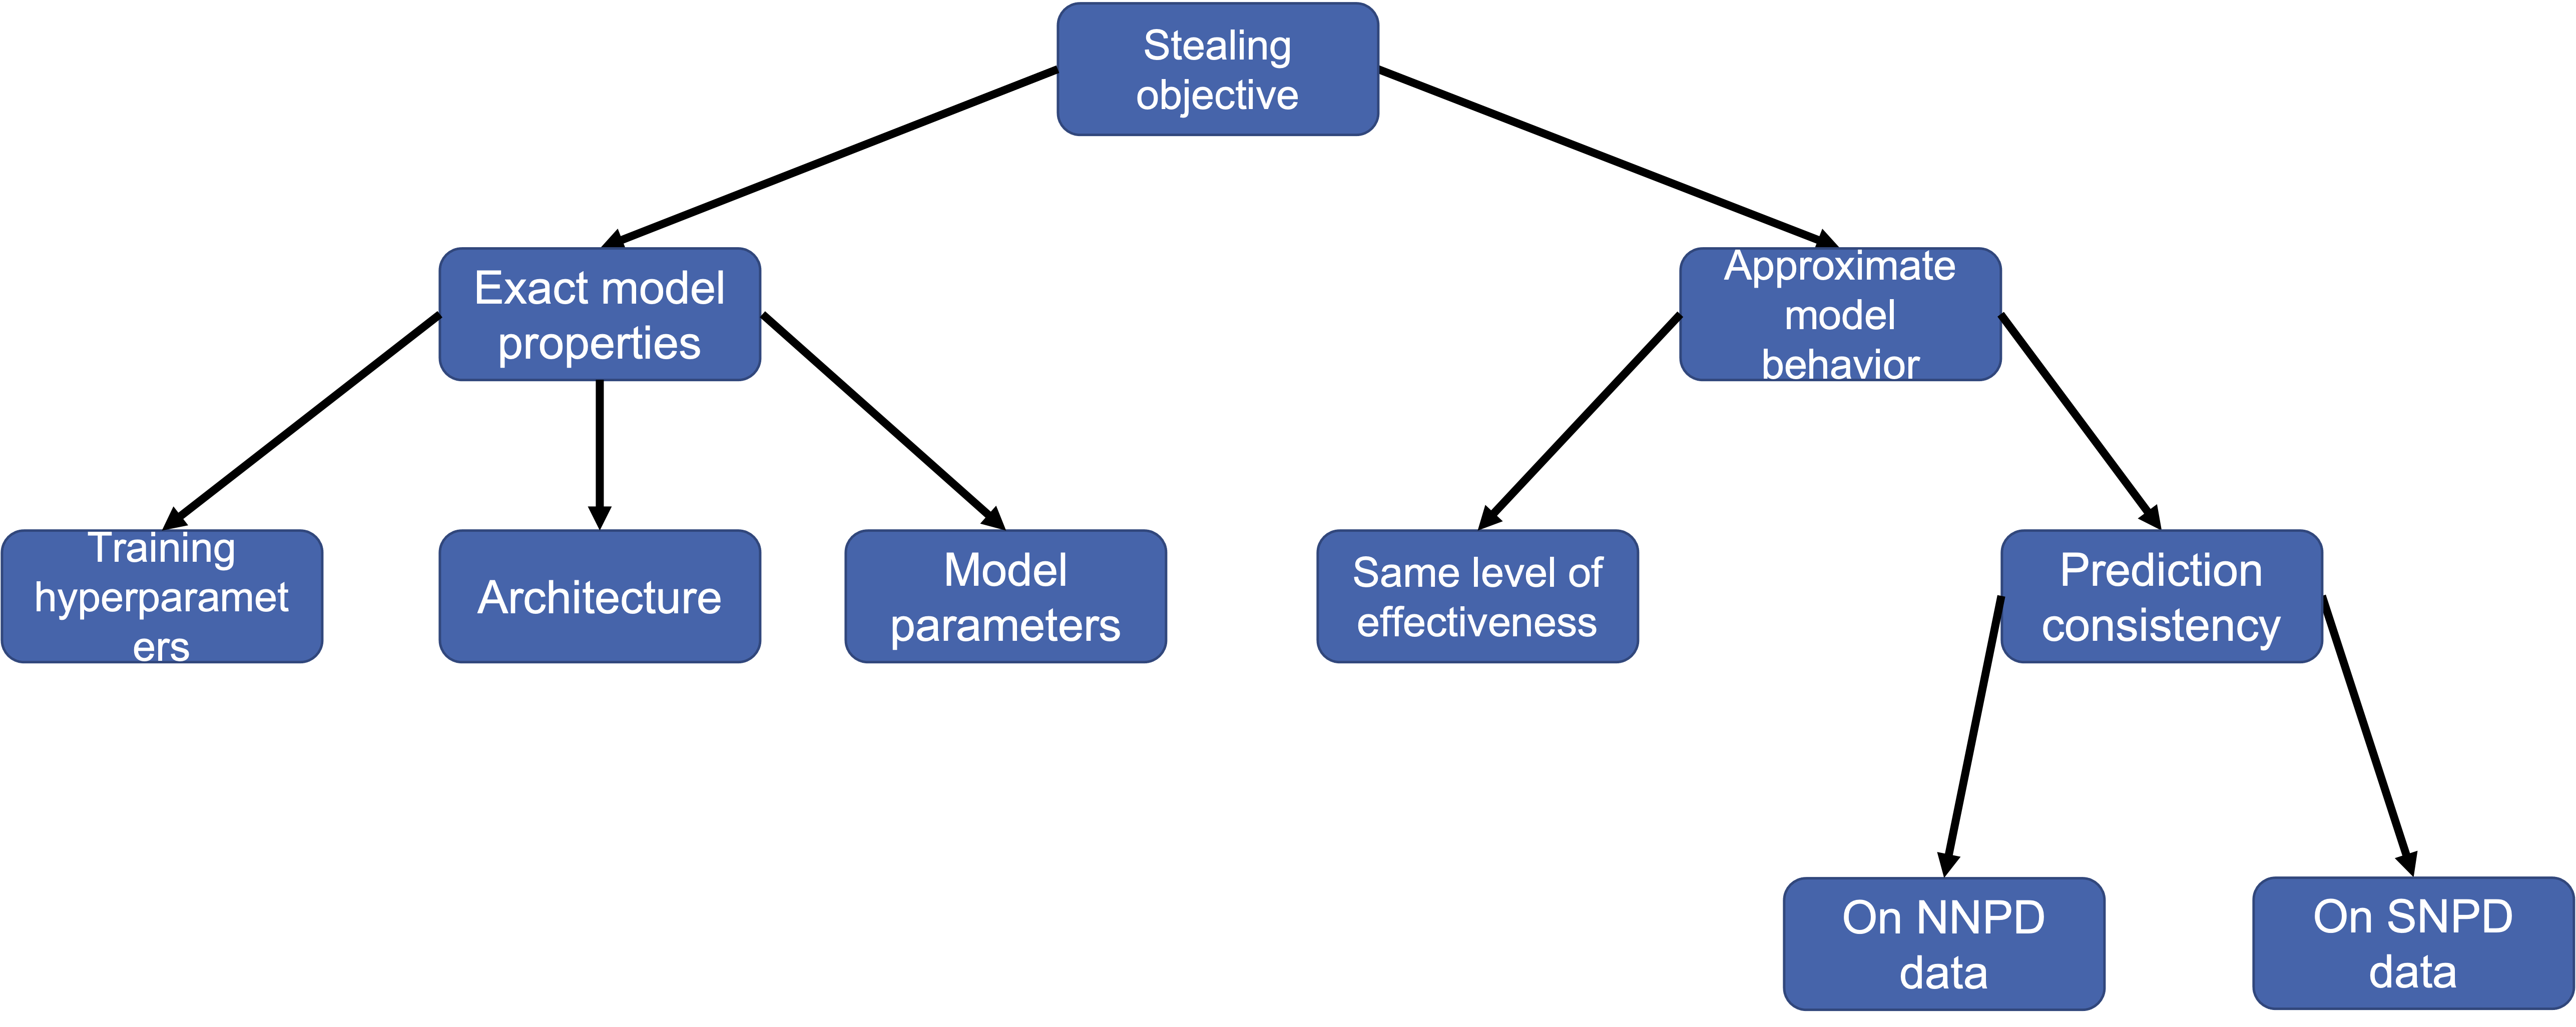
\includegraphics[width=.9\linewidth]{images/MS_Taxonomy.png}
  \caption[Model Stealing Taxonomy]{Taxonomy of Model Stealing Attacks by \cite{oliynyk2022know}}
  \label{fig:ModelStealing:Taxonomy}
\end{figure}


\subsection{Model Stealing Defenses}
\label{sec:ModelStealing:Defenses}
Because of the detrimental effect of Model Stealing Attacks, many defenses have been proposed to protect against them. Defenses can be categorized into proactive and
reactive defenses. While proactive defenses actively aim to prevent or at least complicate Model Stealing Attacks, reactive approaches purely aim to detect them.

\subsubsection{Reactive Model Stealing Defenses (Detection)}
\label{sec:ModelStealing:Defenses:Detection}
Reactive Model Stealing Defenses purely aim to detect Model Stealing Attacks, not prevent them from happening. So far, Model Stealing Detection Approaches
rely either on Watermarking or Monitoring. Watermarking is a way to prove ownership of a Machine Learning model. This is usually achieved by \enquote{hiding} information
in the model which can only be restored by the original owner. A watermark can be a predefined prediction value for outlier samples that are unlikely to be part of the
thief dataset. Watermarking can be applied during training \cite{zhang2018protecting} or afterward \cite{szyller2021dawn}. Monitoring is a way to detect Model Stealing
Attacks by investigating a user's queries to the target model. Kesarwani et al. \cite{kesarwani2018model} proposed a method that estimates the relative amount of the
data space a user has covered with his queries. Based on this metric, they can infer the status of a possible extraction attack. Another approach named \gls{prada} 
\cite{juuti2019prada} analyses the distribution of the samples that a user has queried so far. They assume that the distance between queries of a benign user follows
a normal distribution. Consequently, any user whose query distances are not normally distributed is considered an attacker. \par

\begin{figure} [ht]
    \centering
    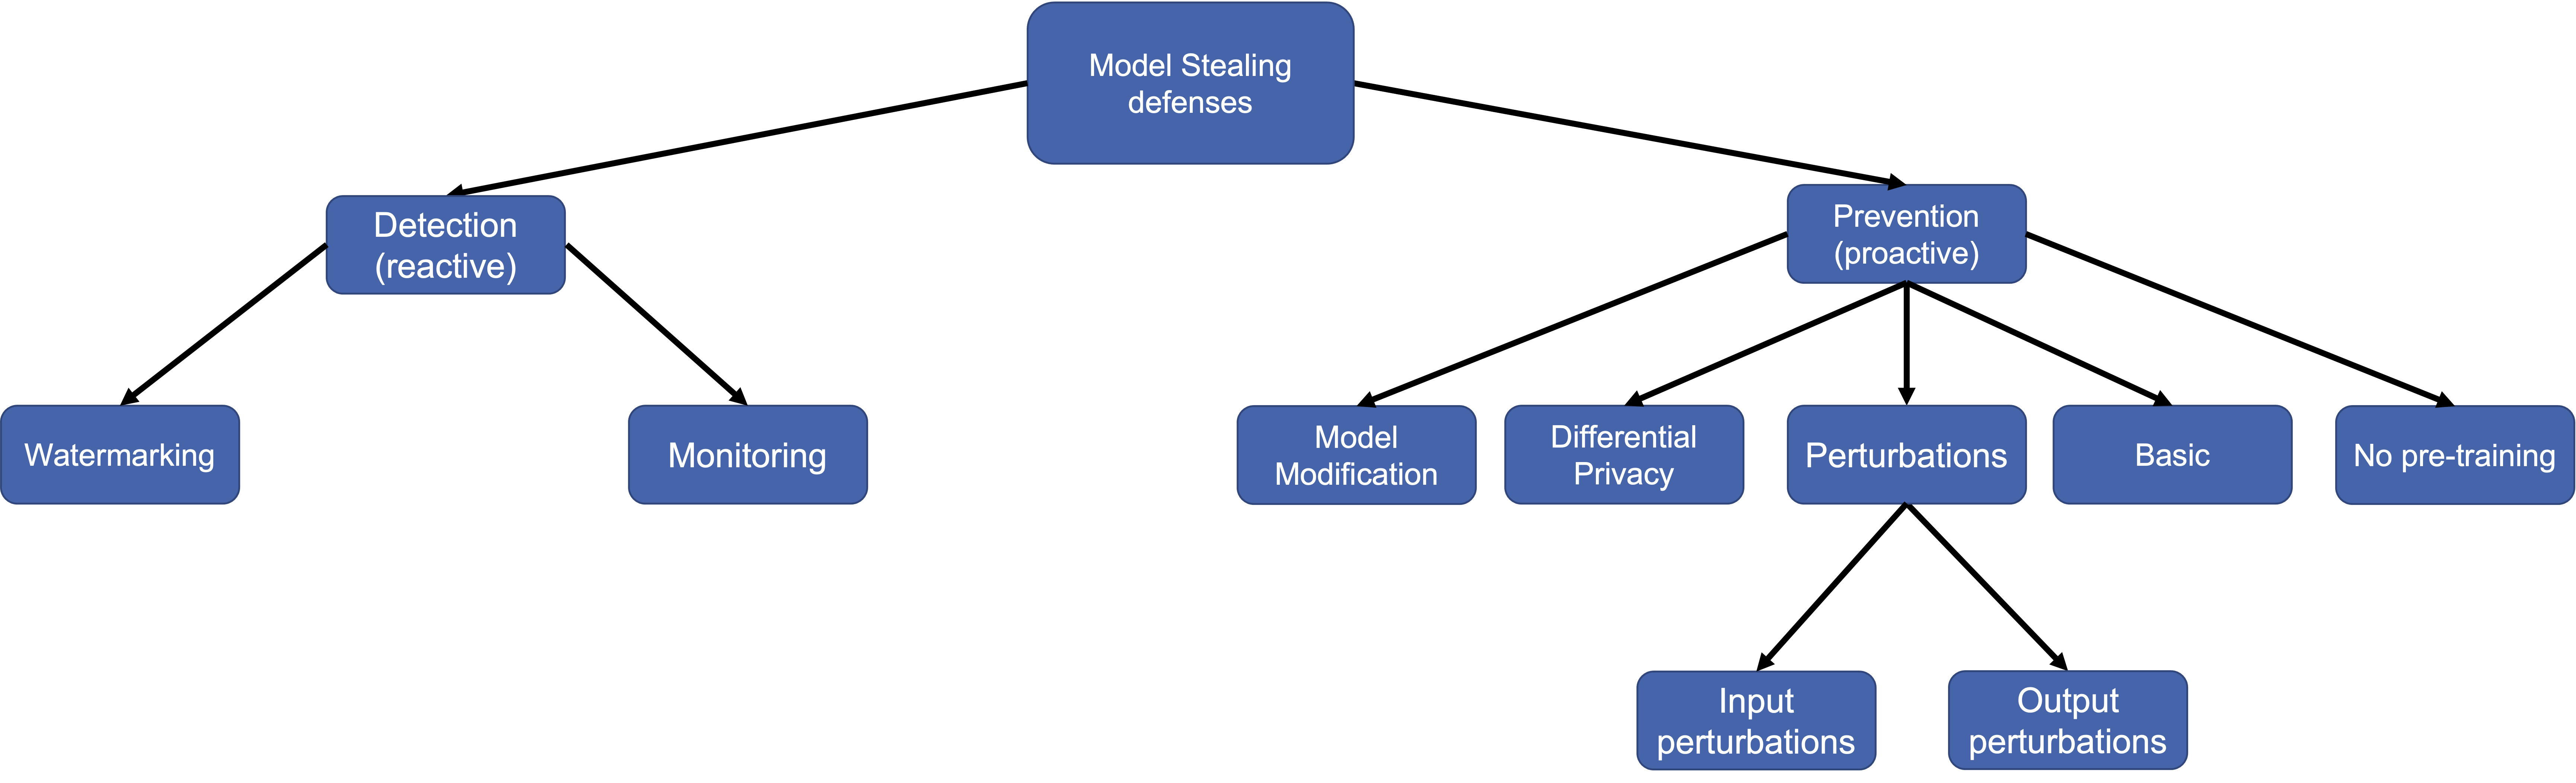
\includegraphics[width=.9\linewidth]{images/MS_defenses_Taxonomy.png}
    \caption[Model Stealing Defenses Taxonomy]{Taxonomy of Model Stealing Defenses by \cite{oliynyk2022know}}
    \label{fig:ModelStealingDefenses:Taxonomy}
  \end{figure}

\subsubsection{Proactive Model Stealing Defenses (Prevention)}
\label{sec:ModelStealing:Defenses:Prevention}
Proactive Model Stealing Defenses aim to complicate or prevent Model Stealing Attacks from happening. It is important to note that the success of a Model Stealing attack is not binary
compared to breaking into a house. Model Stealing Attacks will always be successful to some degree. However, their success mainly depends on the accuracy the substitute model
can achieve (or the achieved model agreement in case the attacker tries to optimize for that). So the quality of a Proactive Model Stealing Defense should be measured by how much it can 
decrease the accuracy of the substitute model compared to a Model Stealing Attack with no defense. A key challenge in developing Proactive Model Stealing Defenses is that, on one hand,
extracting the Target Model should be challenging while on the other hand, the user experience of benign users should not be affected. \par
Early on, a few basic approaches against Model Stealing Attacks were proposed. These include training several models and randomly choosing the output of one of them 
\cite{alabdulmohsin2014adding}. An even simpler albeit effective approach is to output only the predicted label instead of the vector of output probabilities \cite{tramer2016stealing}.
A downside to this is that a benign user loses a lot of information about the output and the model is less interpretable. Another approach of similar complexity is to renounce
using pre-trained models \cite{atli2020extraction} and instead train the target model from scratch. \par
To prevent Model Stealing Attacks, researchers have proposed to use data perturbation. One can either perturb the data fed to the target model or its prediction.
Input perturbation can be performed by adding noise to unimportant pixels determined via Gradient Class Activation Maps \cite{guiga2020neural}. To perform output perturbation,
the developer of the target model can either use Maximizing Angular Deviation (\gls{mad}) \cite{orekondy2019prediction} or flip a few labels to obfuscate the model's decision boundary
\cite{shi2017evasion}. \par
Furthermore, a few approaches bringing Differential Privacy into the Model Stealing domain have been proposed. Differential Privacy is a way to protect the privacy of a dataset so that 
it is impossible for an adversary to determine if a particular individual is part of the dataset. One of these approaches was proposed by Zheng et al. \cite{zheng2019bdpl} who add a so-
called \enquote{Boundary Differential Privacy Layer} to the target model. \par
The final type of Proactive Model Stealing Defense is modifying the target model's architecture. Approaches falling into this category add redundant layers to the target model 
\cite{chabanne2020protection}, propose novel model layers \cite{xu2018deepobfuscation}, or increase model sensitivity \cite{szentannai2020preventing}.
